\documentclass[letterpaper]{article}

\usepackage{aaai}
\usepackage{times}
\usepackage{helvet}
\usepackage{courier}
\usepackage[pdftex,dvipsnames]{xcolor}
\usepackage{xargs}
\usepackage{hyperref}
\usepackage{listings}
\usepackage{multicol}

\usepackage[colorinlistoftodos,prependcaption,textsize=tiny]{todonotes}
\newcommandx{\unsure}[2][1=]{\todo[linecolor=red,backgroundcolor=red!25,textcolor=black,bordercolor=red,#1]{#2}}
\newcommandx{\change}[2][1=]{\todo[linecolor=blue,backgroundcolor=blue!25,bordercolor=blue,#1]{#2}}
\newcommandx{\info}[2][1=]{\todo[linecolor=OliveGreen,backgroundcolor=OliveGreen!25,bordercolor=OliveGreen,#1]{#2}}
\newcommandx{\improvement}[2][1=]{\todo[linecolor=Plum,backgroundcolor=Plum!25,bordercolor=Plum,#1]{#2}}
\newcommandx{\thiswillnotshow}[2][1=]{\todo[disable,#1]{#2}}

\frenchspacing
\setlength{\pdfpagewidth}{8.5in}
\setlength{\pdfpageheight}{11in}
\pdfinfo{
/Title (Finding Parallel Regions with Temporal Planning)
/Author (Claudio Scheer)}
\setcounter{secnumdepth}{0}

\lstdefinestyle{pddlStyle}{
    captionpos=b,
    numbers=left,
    numberstyle=\tiny,
    numbersep=6pt,
    % language=Lisp,
    % xleftmargin=12pt,
    stringstyle=\ttfamily\small,
    basicstyle=\ttfamily\footnotesize,
    showstringspaces=false,
    breaklines,
    % frame=single,
    escapechar=|,
    keywords={
        % at,
        % start,
        % end,
        % forall
    },
    otherkeywords={
        :duration,
        :durative-action,
        :parameters,
        :condition,
        :effect,
        :goal,
        :init
    },
    columns=fullflexible,
}

\lstdefinestyle{cppStyle}{
    captionpos=b,
    numbers=left,
    numberstyle=\tiny,
    numbersep=6pt,
    language=c++,
    % xleftmargin=12pt,
    stringstyle=\ttfamily\small,
    basicstyle=\ttfamily\footnotesize,
    showstringspaces=false,
    breaklines,
    % frame=single,
    escapechar=|,
    columns=fullflexible,
}


\begin{document}

\title{Finding Parallel Regions with Temporal Planning}
\author{Claudio Scheer\\
    Master's Degree in Computer Science\\
    Pontifical Catholic University of Rio Grande do Sul - PUCRS\\
    Porto Alegre - RS, Brazil\\
    claudio.scheer@edu.pucrs.br\\
}
\maketitle

\begin{abstract}
    \begin{quote}
        Testing whether a region in a program can be run in parallel is not an easy task. As an approach to this problem, this paper proposes a formalization of a source code compiler with PDDL. With this approach, it is possible to reduce the identification of parallel regions in a source code to a conventional search problem. The STP planner was used to find a temporal plan in which some actions can be execute in parallel. The results show that temporal planning can be an alternative to find parallel regions, but more studies are still needed, mainly on how to translate a source code to a PDDL problem.
    \end{quote}
\end{abstract}

\noindent There are still many programs that do not exploit the parallel capacity of today's multiprocessors. One of the main reasons for this is because the cost to rewrite a program is high. Among the steps involved in the process of migrating a program to a parallel approach, the most expensive is to identify the regions of the program than can be executed in parallel. In addition to identifying the regions, it is necessary to validate whether the parallel execution of that region brings positive results.

According to \cite{doi:10.1177/1094342017695639}, loops detection, variable dependencies, identifying whether the arguments are read or written, among other analyzes, are the main patterns that identify a region parallel in a program. However, over time, these caracteristics may change and the static analysis will also need to be changed.

Therefore, instead of using a static analysis of the source code, the approach in this paper reduces the problem of identifying a parallel region to a search problem. The compiler domain uses PDDL as a planning representation. In a nutshell, the domain works as a source code compiler and the problem formalization as the source code. The Section~Formalization discusses in more detail how the PDDL domain works.

The PDDL domain describes actions that can be performed in an initial state, to achieve a set of goals. In this paper, the initial state is the dependency tree of the variables and operations of the source code. The set of goals is the complete execution of all instructions in the source code, taking into account the dependency tree.

A problem formalized in PDDL cannot understand source code written in C++ as input. The initial state must be a set of predicates. Hence, the source code provided as the initial state for the planner must be mapped to a set of predicates. This process is the bottleneck of the proposed approach. Some ideas for this problem are discussed in the Section~Source~Code~Translation.

The Section~Bibliography discusses what temporal planning is and some details of the STP planner used. In the Section~Results, I show the results obtained in a real world example. Finally, the Section~Conclusion leaves some questions that still need to be answered in this new approach to find parallel regions.


\section{Bibliography}

\subsection{Temporal Plannign} \label{label:temporal-planning}

According to \cite{DBLP:series/synthesis/2019Haslum}, actions in temporal planning have a duration. Therefore, the planner searches for a schedule in which independent actions can be executed in parallel.

There are different approaches that can be used to formalize temporal actions in PDDL. In this paper, \texttt{:durative-action} was used. Durative actions is represented in the four sections listed below.

\begin{itemize}
    \item \texttt{:parameters}: parameters needed to execute the action;
    \item \texttt{:duration}: time the action takes to run;
    \item \texttt{:condition}: conditions that need to be respected to apply the effects;
    \item \texttt{:effect}: effects that will be applied to the state;
\end{itemize}

The sections \texttt{:condition} and \texttt{:effect} are separated in three categories: \texttt{at start}, \texttt{over all} and \texttt{at end}. As described by \cite{DBLP:series/synthesis/2019Haslum}, these categories represent the conditions and effects used at each stage of the durative action. The \texttt{at start} statements are used when starting the action. The \texttt{over all} statements are used during the time the action is being executed. The \texttt{at end} statements are used at the end of the action.

\subsection{STP}

The STP (Simultaneous Temporal Planner) planner, introduced by \cite{Blanco2018ForwardsearchTP}, was used to find the best temporal plan for a problem. STP is a modified version of the Fast Downward \cite{Helmert_2006} planner that allows solving temporal planning problems. The version used in this paper is provided by the Artificial Intelligence and Machine Learning Group - Universitat Pompeu Fabra\footnote{\href{https://github.com/aig-upf}{https://github.com/aig-upf}}.

The STP planner receive as a parameter the maximum number of actions that can be executed at the same time. When finding parallel regions, this parameter is a problem, because we do not know how many instructions can be executed in parallel. Therefore, in some cases, it is necessary to test different values for this paramenter. It is important to note that the higher this number, the longer the STP planner takes to find a temporal plan.


\section{Source Code Translation}

The correct translation of the source code is the main point to find parallel regions using temporal planning. And, this paper do not cover all the possibilities in a source code. The focus is on source codes with assignments and operations between two variables and simple loops.

It is easy to formalize in a PDDL problem a source code without loops. The dependency tree is easy to create. More about these type of problems is discussed in Section~Results.

However, when the source code has a loop, the level of abstractions becomes an issue. For example: is it necessary to formalize the assignments that control the index of a for loop? Two examples of a for loop in C++ are shown below.

The Listing~\ref{lst:sum-vector-cpp} shows an algorithm that adds up all the items in a vector. In this case, the variable \texttt{i} accesses different loctions of the vector. In theory, the sum of \texttt{s} plus \texttt{x[i]} can be executed in parallel. Since the order of a sum does not matter and \texttt{s} is shared between threads\footnote{The concurrency between variables is not taked into account here.}, in the end, \texttt{s} will be equal to 6.

\begin{lstlisting}[caption=Sum of vector - C++,label=lst:sum-vector-cpp,style=cppStyle]
int main()
{
    int s = 0;
    std::vector<int> x = {1, 2, 3};
    for (int i = 0; i < x.size(); i++)
    {
        s += x[i];
    }
    return 0;
}
\end{lstlisting}

In the formalization of the Listing~\ref{lst:sum-vector-cpp}, the assignment of the variable \texttt{i} can be ignore. However, in the Listing~\ref{lst:initializing-array-cpp}, where the initialization of a position in the array depends on the value of the previous position, the variable \texttt{i} cannot be ignored. If the loop is executed in parallel, the previous position may not have been initialized yet, throwing an exception.

\begin{lstlisting}[caption=Initializing array - C++,label=lst:initializing-array-cpp,style=cppStyle]
int main()
{
    int a[3] = {0};
    a[0] = rand();
    for (int i = 1; i < 3; ++i)
    {
        a[i] = a[i - 1] + rand();
    }
    return 0;
}
\end{lstlisting}

There are many variants that can happen in a source code an the level of abstraction depends on how the program was built.


\section{Formalization}

Two \texttt{:durative-action} were used to formalize the PDDL domain. One to handle assignment instructions and another to handle binary operations. Binary operations must be understood as any operations (sum, multiplication, XOR, etc) that involve two variables.

All \texttt{:durative-action} must have a duration time. However, since the goal is not to cover the execution time for specific instructions, the duration was set to 1 for all actions. This approach ensures that when operations cannot be executed in parallel, the total execution time will be increased by one. In future work, it may be a good approach to define a different time for each instruction.

By definition, each operation and assignment instruction must have an identifier. With the identification, the instructions dependency tree can be created. The dependency tree makes it easy to test whether all dependencies for a specific instruction have already been executed or not. As each problem has a specific dependency tree, the dependency tree must be defined in the initial state of the problem. In addition to the dependency tree, the identifier of the binary operations and assignments must also be defined in the initial state.

As discussed in Section~Temporal~Plannign, the sections \texttt{:conditions} and \texttt{:effects} have three different categories. In the proposed formalization, all preconditions must be respected at the beginning of the action and the effects is applied only at the end of the action.

\subsection{Assignment Action}

The assignment action will receive the assignment instruction and the instruction identifier as parameters. The first two conditions will ensure that the identifier belongs to the the instruction and that the assignment has not yet been executed.

The third condition is common the all durative actions. The \texttt{forall} operator loops through all identifiers in the dependency tree, testing whether the identifier is the parent of the current instruction and whether the parent instruction has already been executed.

The Table~\ref{table:forall-truth-table} shows the truth table that represents the condition in the \texttt{forall} operator. The variable $A$ represents that the current identifier is a child of the parent identifier. $B$ represents that the parent identifier has already been executed. As shown in the truth table, the only case where the condition returns false is when the current identifier is a child of the parent identifier and the instruction represented by the parent identifier has not yet been executed.

\begin{table}[h]
    \centering
    \begin{tabular}{|c|c|c|}
        \hline
        $A$ & $B$ & $\neg A \lor B$ \\
        \hline
        1   & 1   & 1               \\
        1   & 0   & 0               \\
        0   & 1   & 1               \\
        0   & 0   & 1               \\
        \hline
    \end{tabular}
    \caption{Dependency tree condition truth table}
    \label{table:forall-truth-table}
\end{table}

The \texttt{:effect} of the assignment action is to mark the instructions as executed. The Listing~\ref{lst:assignment-action} shows the formalization of the assignment action.

\begin{lstlisting}[caption=Formalization of the assignment action,label=lst:assignment-action,style=pddlStyle]
(:durative-action assignment
    :parameters (
        ?instruction_id - id
        ?id - assignment
    )
    :duration (= ?duration 1)
    :condition (and
        (at start (assignment_id ?id ?instruction_id))
        (at start (not (executed_assignment ?id)))
        (at start (forall (?parent - id)
            (or
                (not (dependency_tree ?parent ?instruction_id))
                (executed_instruction ?parent)
            )
        ))
    )
    :effect (and
        (at end (executed_instruction ?instruction_id))
        (at end (executed_assignment ?id))
    )
)
\end{lstlisting}

\subsection{Binary Operation Action}

This action is responsible for executing a binary operation between two variables. The action takes as parameters the two assignment variables that will be used in the operation and the assignment instruction that will receive the result of the binary operation.

The conditions to execute the action are that the binary operation has not yet been executed and the assignment instructions of the two input variables have already been executed.

As shown in Listing~\ref{lst:binary-operation-action}, the effects are similar to the previous action: the binary operation is marked as executed, releasing the next instructions that holds in this operation.

\begin{lstlisting}[caption=Formalization of the binary operation action,label=lst:binary-operation-action,style=pddlStyle]
(:durative-action binary_operation
    :parameters (
        ?instruction_id - id
        ?idA - assignment
        ?idB - assignment
        ?operation_id - operation
        ?idC - assignment
    )
    :duration (= ?duration 1)
    :condition (and
        (at start (operation_id ?operation_id ?instruction_id))
        (at start (forall (?parent - id)
            (or
                (not (dependency_tree ?parent ?instruction_id))
                (executed_instruction ?parent)
            )
        ))
        (at start (not (executed_operation ?operation_id)))
        (at start (not (executed_binary_operation ?idA ?idB ?operation_id ?idC)))
        (at start (executed_assignment ?idA))
        (at start (executed_assignment ?idB))
    )
    :effect (and
        (at end (executed_instruction ?instruction_id))
        (at end (executed_operation ?operation_id))
        (at end (executed_binary_operation ?idA ?idB ?operation_id ?idC))
    )
)
\end{lstlisting}


\section{Results}

In this section, the results achieved are discussed. Loops are not shown in the results because more research is still needed to better understand how to abstract the set of predicates from a source code. Therefore, with regard to the objective of the paper, it is expected that the temporal plan found by the planner shows the instructions that can be execute in parallel. In Listing~\ref{lst:source-code}, the source code used in the examples discussed is presented. The source code is simple, but it will help to show the capacity of the proposed approach.

The source code in Listing~\ref{lst:source-code} adds two variables and store the result in the variable \texttt{c}. The variables \texttt{a} and \texttt{b} are not dependent on each other. Therefore, the two assignment instructions can be executed in parallel, as shown in Figure~\ref{fig:dependency-tree-parallel}.

\begin{lstlisting}[caption=Source code,label=lst:source-code,style=cppStyle]
int main()
{
    int a = 3;
    int b = 3;
    int c = a + b;
    return 0;
}
\end{lstlisting}

\begin{figure}[h]
    \centering
    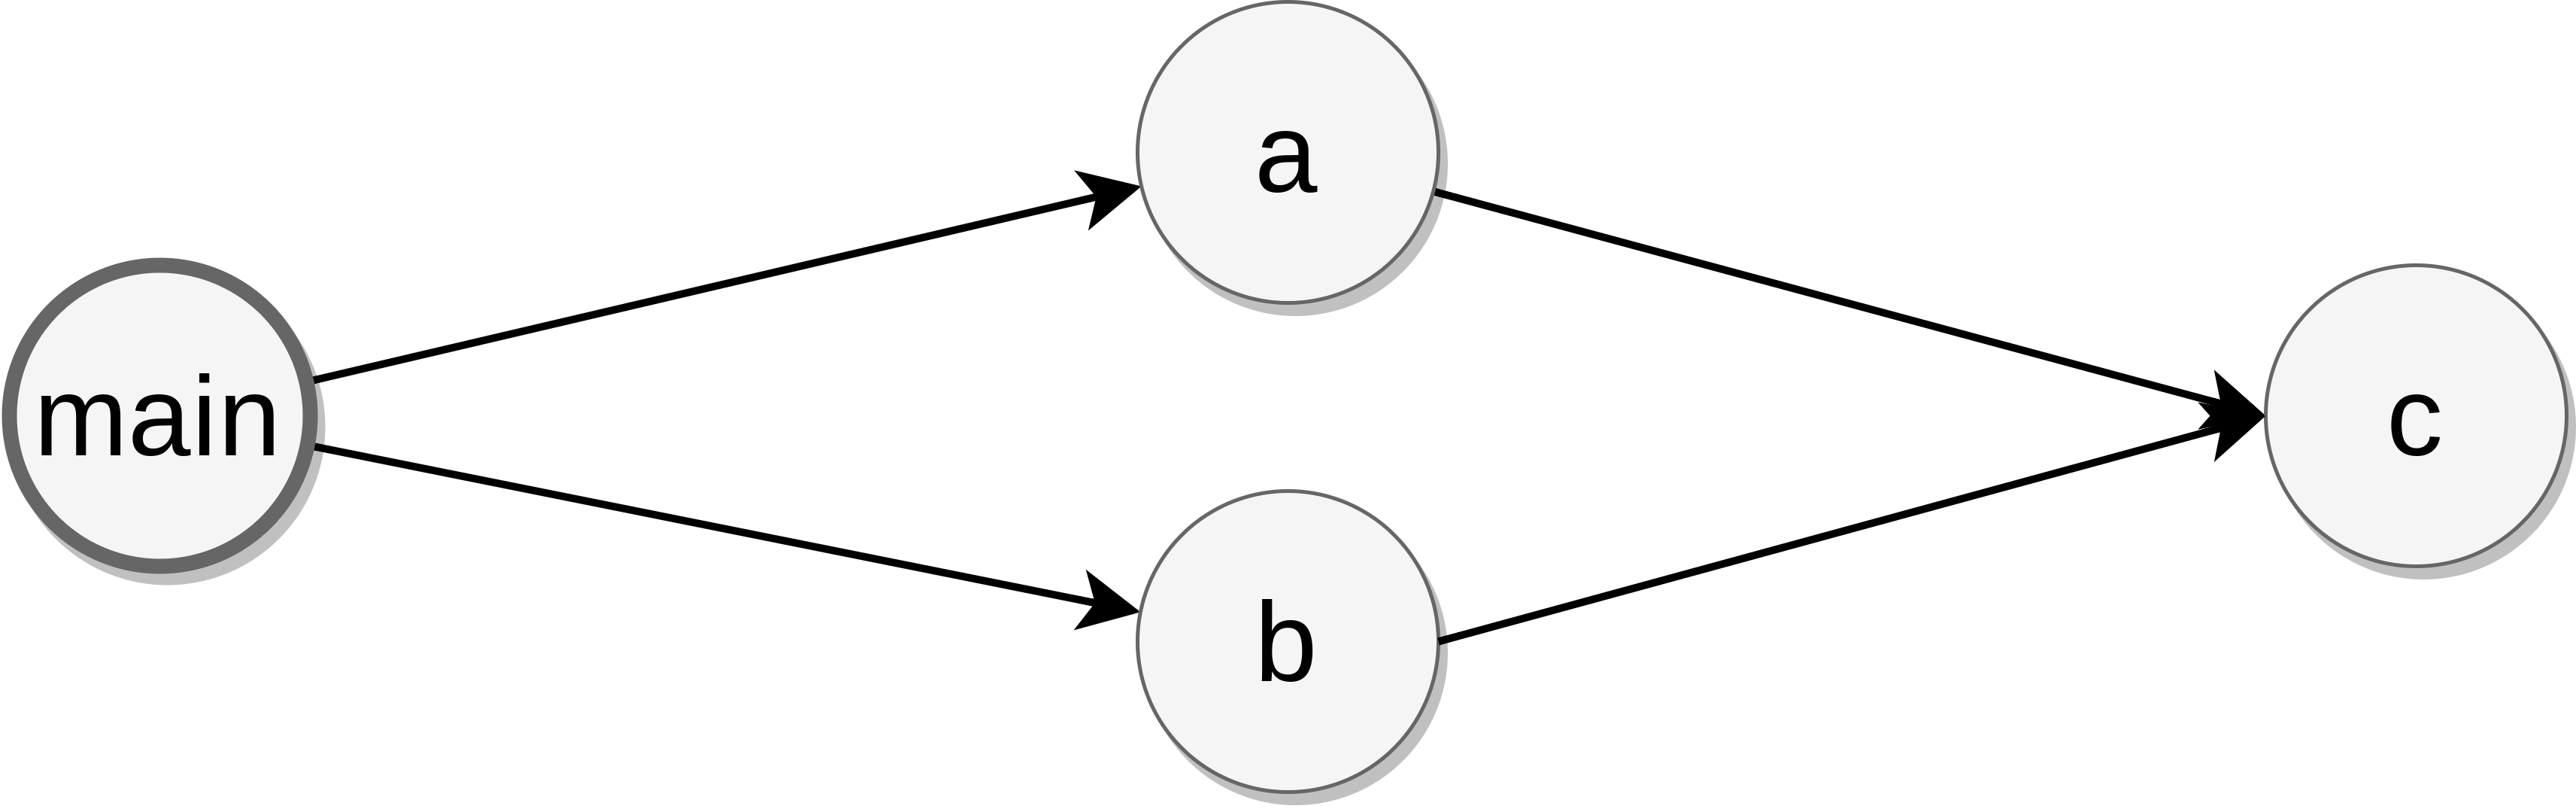
\includegraphics[width=0.4\textwidth]{./images/dependency-tree-Parallel.png}
    \caption{Dependency tree}
    \label{fig:dependency-tree-parallel}
\end{figure}

The formalization of the Listing~\ref{lst:source-code} is shown in Listing~\ref{lst:source-code-formalization}.

\begin{lstlisting}[caption=Source code formalization,label=lst:source-code-formalization,style=pddlStyle]
(:init
    (executed_instruction id0)

    (assignment_id assignmentA id1)
    (assignment_id assignmentB id2)
    (operation_id sumAB id3)
    (assignment_id assignmentC id4)
    
    (dependency_tree id0 id1)
    (dependency_tree id0 id2)
    (dependency_tree id1 id3)
    (dependency_tree id2 id3)
    (dependency_tree id3 id4)
)

(:goal (and
    (executed_assignment assignmentA)
    (executed_assignment assignmentB)
    (executed_binary_operation assignmentA assignmentB sumAB assignmentC)
    (executed_assignment assignmentC)
))
\end{lstlisting}

The main point in Listing~\ref{lst:source-code-formalization} is on lines 9 and 10. In these lines, the instructions \texttt{a} and \texttt{b} are defined as dependent only on the main instruction\footnote{The main instruction represents the starting point of the application. In this example, \texttt{id0}.}. The STP output of this formalization is represented visually in Figure~\ref{fig:parallel-plan}.

\begin{figure}[h]
    \centering
    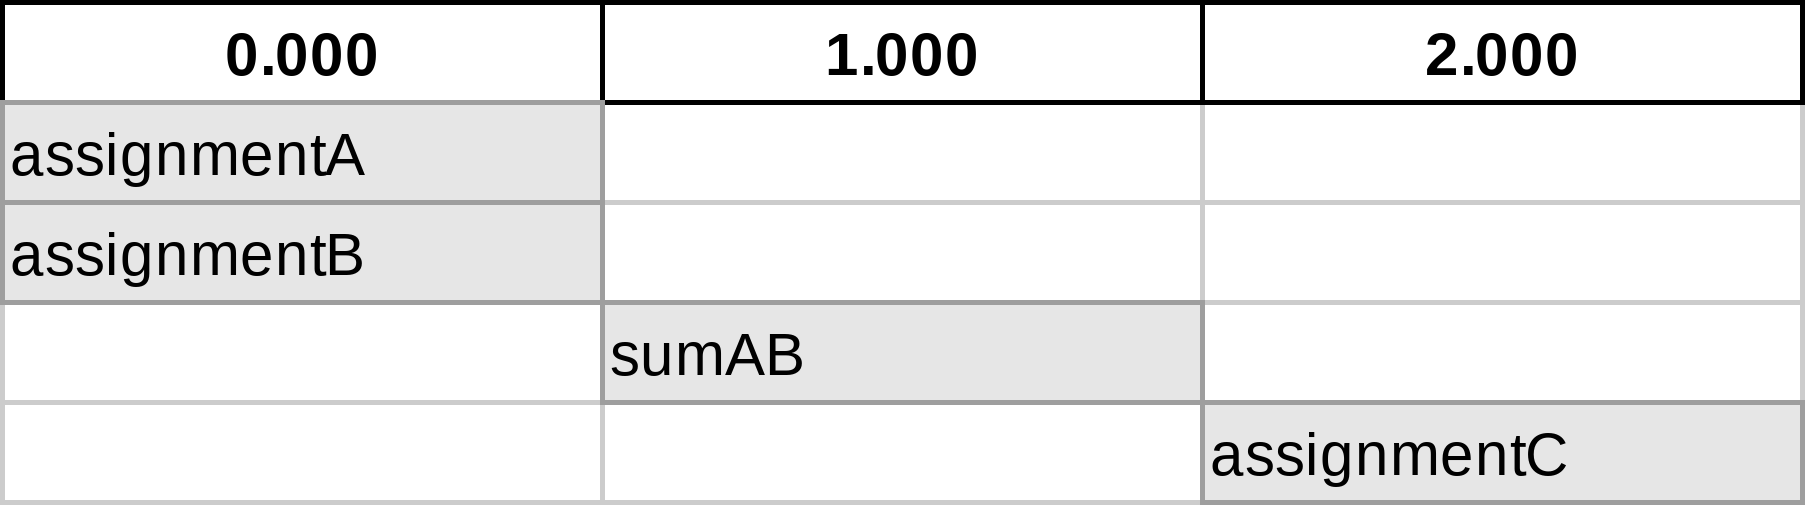
\includegraphics[width=0.4\textwidth]{./images/parallel-tasks-Parallel.png}
    \caption{STP parallel plan}
    \label{fig:parallel-plan}
\end{figure}

Figure~\ref{fig:parallel-plan} shows that, as soon as the program starts, the instructions \texttt{assignmentA} and \texttt{assignmentB} can be executed at the same time. However, to execute the \texttt{sumAB} instruction, it is necessary to wait until the previous instructions are executed. Finally, to execute the \texttt{assignmentC} instruction, all previous instructions must be executed.

Imagining a source code similar to Listing~\ref{lst:source-code}, where the variable \texttt{b} is a result of the variable \texttt{a} plus 1, the dependency tree would be different. Now, line 10 in Listing~\ref{lst:source-code-formalization} will be replaced by \texttt{(dependency\_tree\ id1\ id2)}, ensuring that variable \texttt{b} is assigned only after the variable \texttt{a}. The output of this second example is shown in Figure~\ref{fig:not-parallel-plan}.

\begin{figure}[h]
    \centering
    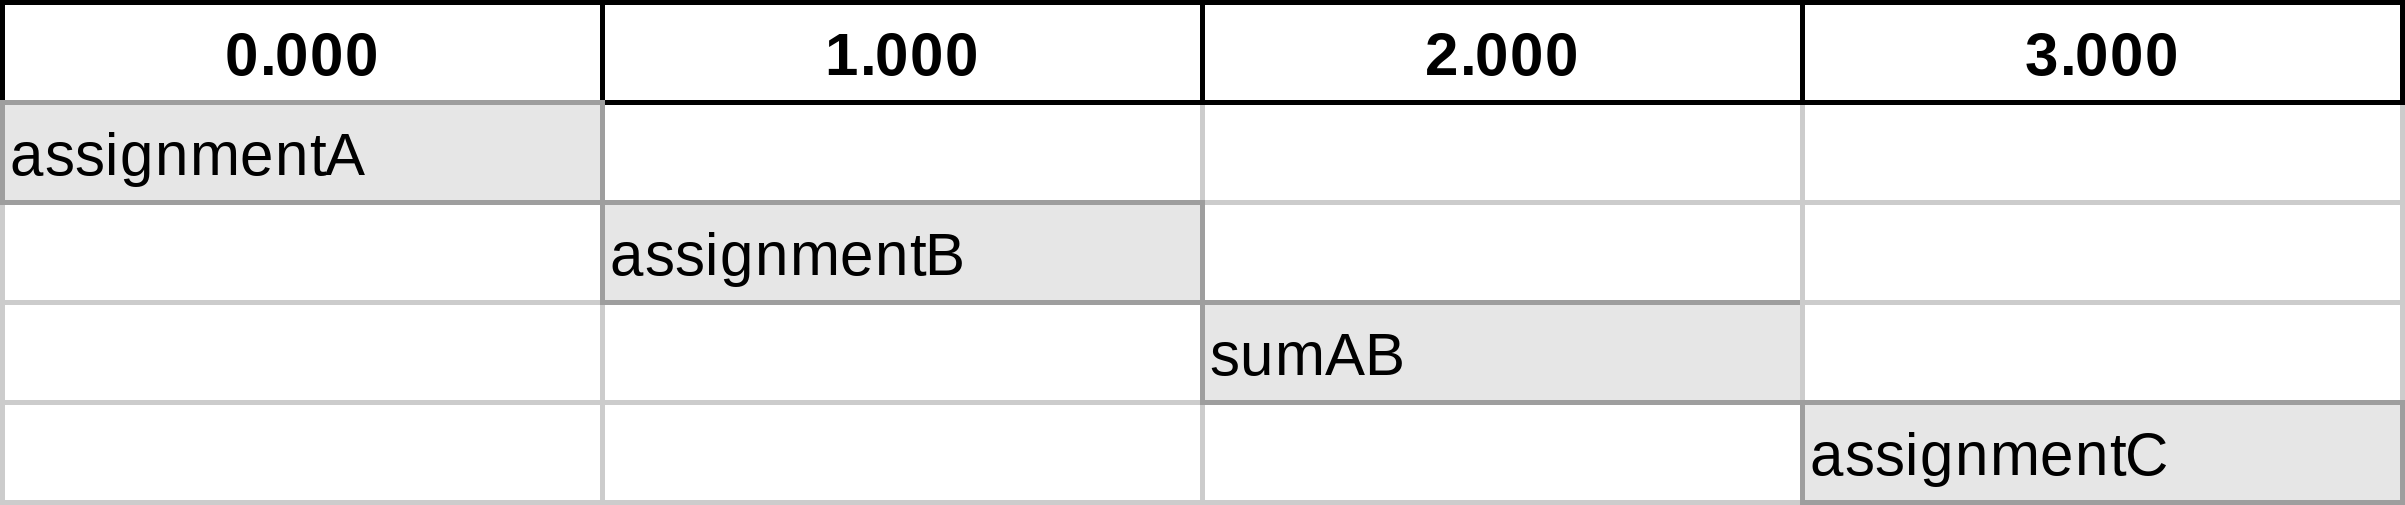
\includegraphics[width=0.43\textwidth]{./images/parallel-tasks-NotParallel.png}
    \caption{STP non-parallel plan}
    \label{fig:not-parallel-plan}
\end{figure}


\section{Conclusion}

The idea of reducing the search for parallel regions in a source code to a search problem is unconventional. Therefore, there are still many questions to be answered:

\begin{itemize}
    \item What is the best way to abstract a source code?
    \item How can nested loops be abstracted?
    \item In a for loop, for example, when should formalization take into account the index assignment (usually the variable \texttt{i})?
    \item Are the two durative actions defined in this paper sufficient?
    \item Can the temporal plan be mapped back to the source code?
    \item How to choose the maximum number of parallel instructions in STP correctly?
    \item Is STP the best temporal planner for this problem?
    \item Shouldn't different duration times be used for each assignment and binary operation?
    \item Do all regions need to run in parallel?
    \item How should \texttt{if} instructions be handled?
\end{itemize}

Despite all these question, there is a guarantee: this approach can identify parallel regions. In addition, the possibility of abstracting the source code to a set of predicates allows to reduce the problem to the same proprierties, but with lower overheads.


\bibliographystyle{aaai}
\bibliography{references}

\end{document}